%
% TAZ-1.tex
%
% History of LulzBot Printers
%
% Copyright (C) 2014, 2015 Aleph Objects, Inc.
%
% This document is licensed under the Creative Commons Attribution 4.0
% International Public License (CC BY-SA 4.0) by Aleph Objects, Inc.
%

\section{LulzBot TAZ-1}
LulzBot TAZ-1.

\begin{figure}[h!]
\thisfloatpagestyle{empty}
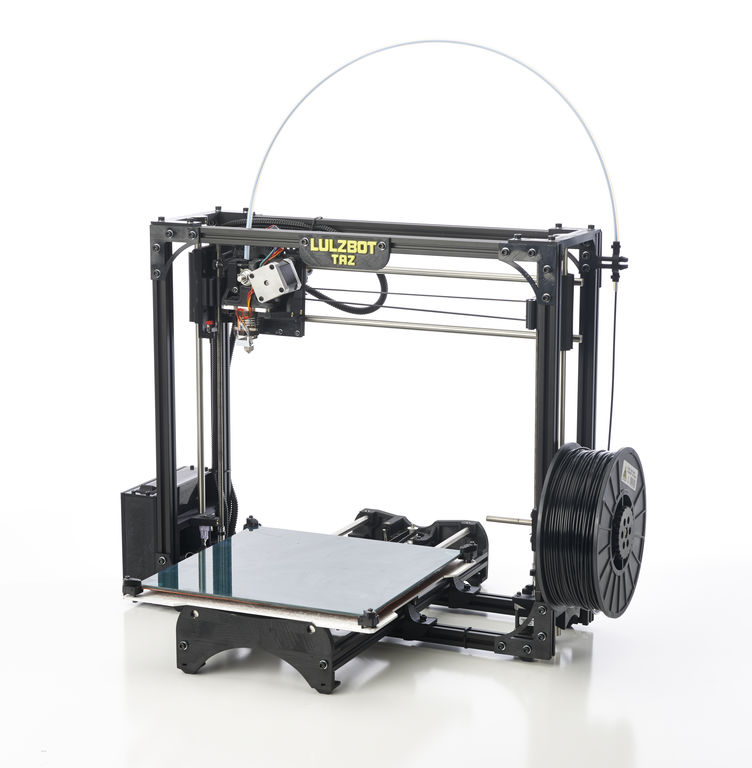
\includegraphics[keepaspectratio=true,height=0.40\textheight,width=1.00\textwidth,angle=0]{taz/taz-1.jpg}
 \caption{LulzBot TAZ-1}
 \label{fig:taz-1}
\end{figure}

\begin{figure}[h!]
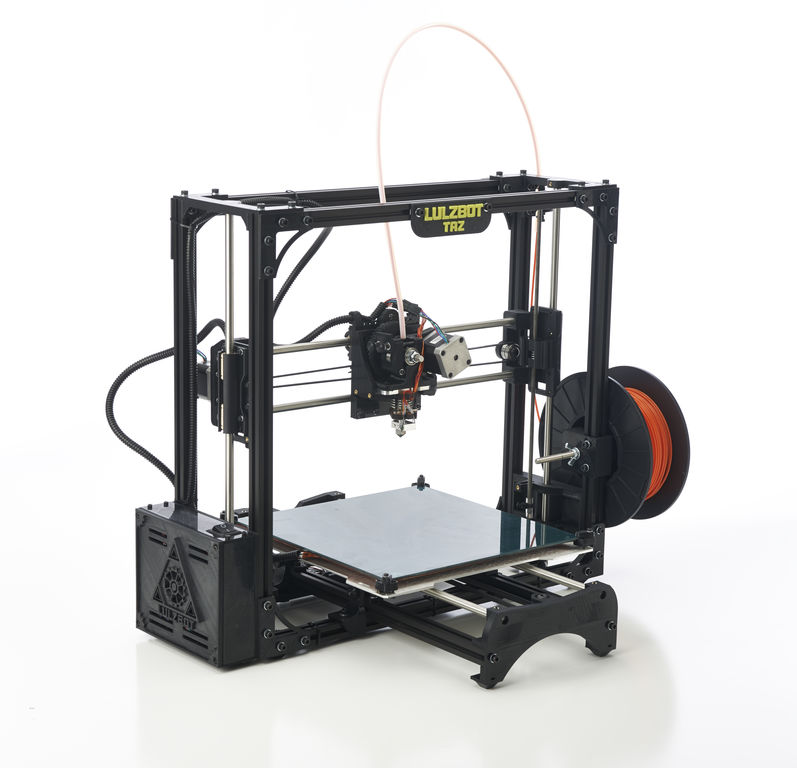
\includegraphics[keepaspectratio=true,height=0.40\textheight,width=1.00\textwidth,angle=0]{taz/taz-1-front-left.jpg}
 \caption{LulzBot TAZ-1 Front Left}
 \label{fig:taz-1-front-left}
\end{figure}

\begin{figure}[h!]
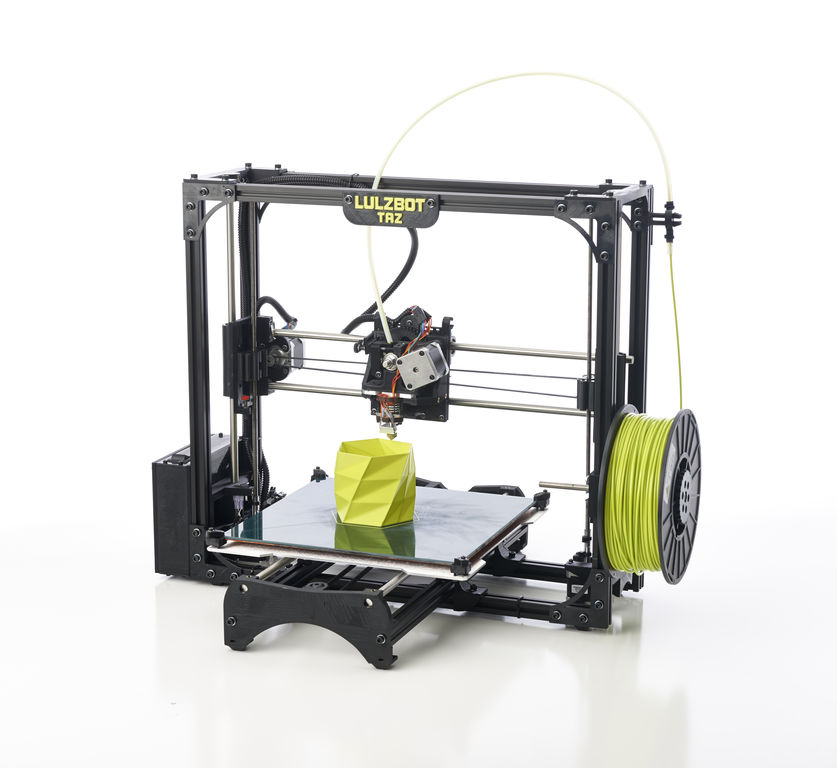
\includegraphics[keepaspectratio=true,height=0.40\textheight,width=1.00\textwidth,angle=0]{taz/taz-1-vase.jpg}
 \caption{LulzBot TAZ-1 with Vase}
 \label{fig:taz-1-vase}
\end{figure}

\begin{figure}[h!]
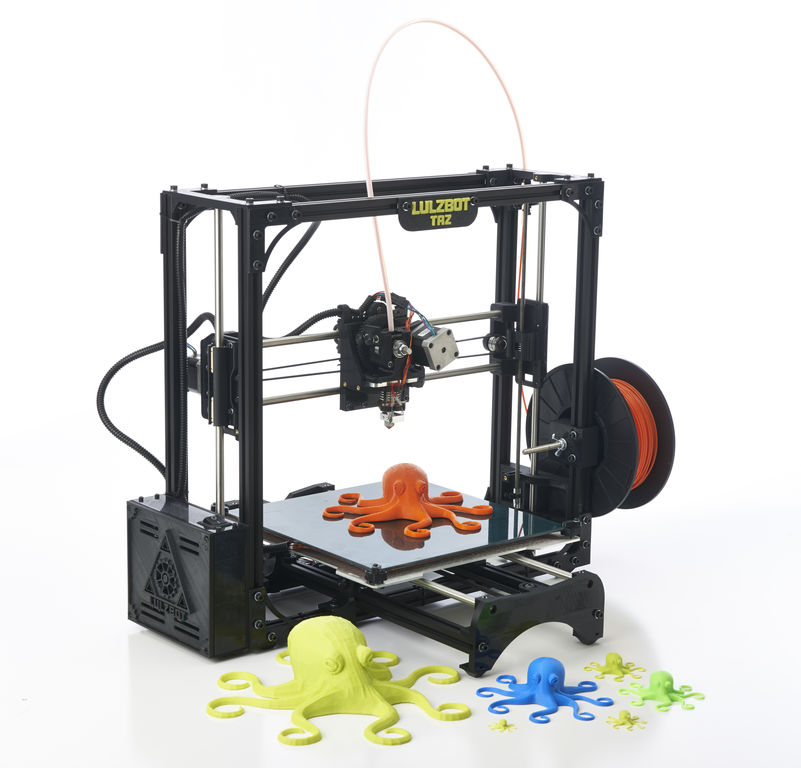
\includegraphics[keepaspectratio=true,height=0.40\textheight,width=1.00\textwidth,angle=0]{taz/taz-1-octo.jpg}
 \caption{LulzBot TAZ-1 with Octopus}
 \label{fig:taz-1-octo}
\end{figure}

\begin{figure}[h!]
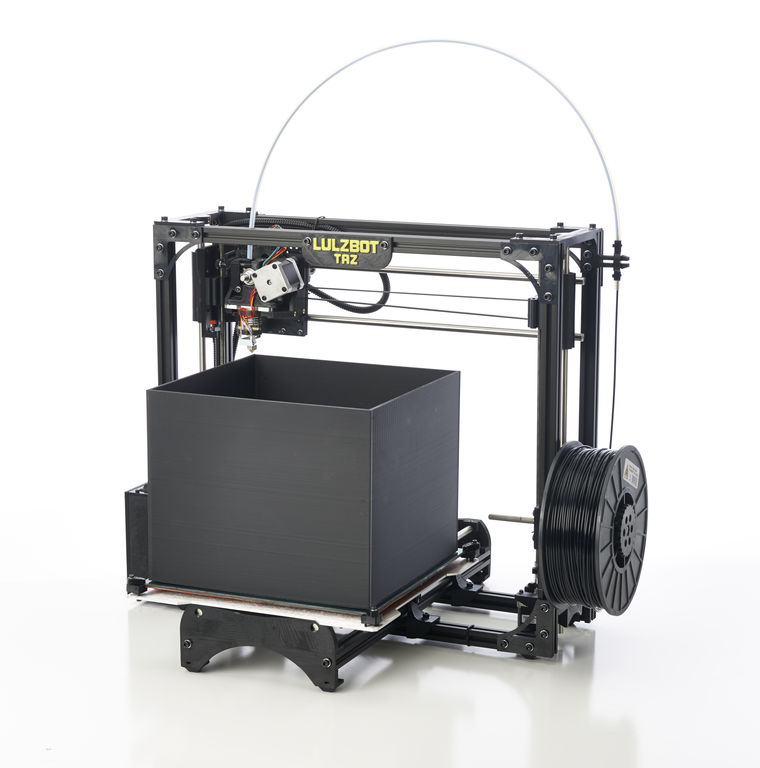
\includegraphics[keepaspectratio=true,height=0.40\textheight,width=1.00\textwidth,angle=0]{taz/taz-1-max.jpg}
 \caption{LulzBot TAZ-1 Max Build Volume}
 \label{fig:taz-1-max}
\end{figure}
